\documentclass[10pt]{beamer}
\usepackage{preamble}
\usetheme{metropolis}
\usepackage{appendixnumberbeamer}
\usepackage{animate}
\usepackage{media9}
\title{Getting Started with \text{\LaTeX}}
\subtitle{And why I don't use Word anymore}
\date{\today}
\author{Jack Naylor}
\institute{Treasurer - PhySoc, University of Sydney}
\titlegraphic{\hfill\includegraphics[height=2cm]{reclogo.png}\flushright\includegraphics[height=1cm]{aiaa-logo-blue.png}}
\begin{document}

\maketitle
\section{What is \text{\LaTeX}?}
\begin{frame}{A bit of Background}
    \begin{itemize}
\item Widely regarded as the standard typesetting method for academic journals
\begin{itemize}
\item Far easier to present data, equations
\item Much easier to cite references (i.e. automatic footnotes, hyperlinking etc.)
\item Separates content from the formatting of documents
\end{itemize}
\item Far more control over many aspects of the document
\begin{itemize}
\item Backend rather than frontend (e.g. Word)
\item Images won't disappear when moved slightly
\begin{itemize}
\item Everything is where you tell it to be
\end{itemize}
\end{itemize}
\end{itemize}
\end{frame}
\begin{frame}
\begin{itemize}
\item Files can be as big as needed, don't need to worry about a 30+ page Word doc crashing
\item Multi-file documents are very easy to achieve, no post-processing
\item It looks \alert{pretty}
\end{itemize}
\end{frame}
\begin{frame}
\centering
Something to keep in mind throughout this presentation: \emph{\alert{every single slide} is done in \LaTeX}
\end{frame}
\section{What can I do?}
\begin{frame}
\centering
    In short: anything you can do with Word + much much more!!
\end{frame}
\begin{frame}{Images}
   \begin{figure}
\centering
\includegraphics[width=\textwidth]{ariba}
\end{figure}
\end{frame}
\begin{frame}
Diagrams from scratch:
    \begin{figure}
        \centering
        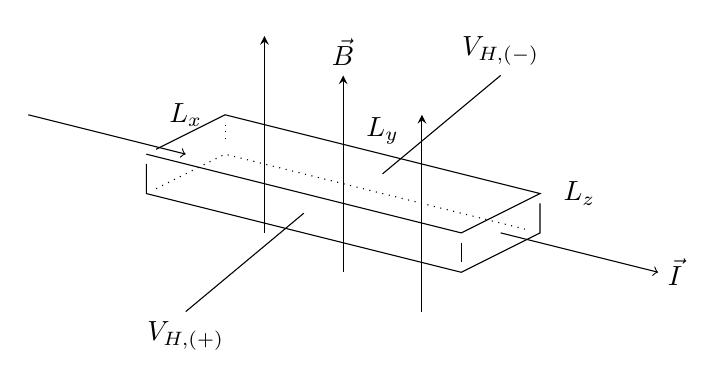
\begin{tikzpicture}
\draw (-1.5,2) node (v1) {} -- (2.5,1) node (v7) {} -- (3.5,1.5) node (v2) {} -- (-0.5,2.5) node (v5) {} -- (v1) -- (-1.5,1.5) node (v3) {} -- (2.5,0.5) node (v8) {} -- (3.5,1) node (v4) {} -- (v2);
\node[above] (v9) at (1.5,2) {$L_y$};
\node at (4,1.5) {$L_z$};
\node at (-1,2.5) {$L_x$};
\draw[->] (3,1) -- (5,0.5);
\draw[<-] (-1,2) -- (-3,2.5);
\draw[dotted] (v3) -- (-0.5,2) node (v6) {} -- (v4);
\draw[dotted] (v5) -- (v6);
\draw (v7) -- (v8);
\draw (0.5,1.25) -- (-1,0);
\draw (1.5,1.75) -- (3,3);
\node[below] at (-1,0) {$V_{H,(+)}$};
\node[above] at (3,3) {$V_{H,(-)}$};
\node[right] at (5,0.5) {$\vec{I}$};
\draw[-stealth] (0,1) -- (0,3.5);
\draw[-stealth] (1,0.5) -- (1,3);
\draw[-stealth] (2,0) -- (2,2.5);
\node[above] at (1,3) {$\vec{B}$};
\end{tikzpicture}
\caption{Semiconductor sample in $B$ field}

    \end{figure}
\end{frame}
\begin{frame}
GIFS:
    \begin{figure}
\animategraphics[loop,autoplay,scale=1]{7}{elon/new-}{0}{76}
\end{figure}
\end{frame}
\begin{frame}
\centering
    \includegraphics[width=\textwidth]{oohyeah}
\end{frame}
\begin{frame}{Maths}
\begin{itemize}
    \item Inline:\\
    It is known that $y=x^2+2x+4$ is a parabola.\par
    \item Block:\\
    Here is a Fourier transform:
    \[\mathcal{F}\left(\omega\right)=\int_{-\infty}^\infty f(t) e^{i\omega t}\dd t\]
    \item Numbered:
    \begin{subequations}
    \begin{align}
        \ket{+_x} &= \frac{1}{\sqrt{2}} \ket{+} + \frac{1}{\sqrt{2}} \ket{-}\\
        \ket{-_x} &= -\frac{1}{\sqrt{2}} \ket{+} + \frac{1}{\sqrt{2}} \ket{-}\\
        \abs{\braket{+}{+_x}}^2 &= 0.5
    \end{align}
    \end{subequations}
\end{itemize}

\end{frame}
\begin{frame}{Plots}
Using gnuplot:
\begin{figure}
\centering
\begin{tikzpicture}[scale=0.8]
\begin{axis}[xlabel = x,
            ylabel = y]
\addplot gnuplot {sin(x)};
\addlegendentry{$y=\sin(x)$}
\end{axis}
\end{tikzpicture}
\end{figure}
\end{frame}
\begin{frame}
\begin{figure}
\centering
\begin{tikzpicture}[scale=1.75]
\begin{axis}[axis equal image,axis lines=none,view={150}{40},]
\addplot3 [raw gnuplot,mesh] gnuplot [mesh]{
   set parametric;
   set pm3d explicit;
   set pal rgb 9,9,3;
   set hidden3d;
   set isosamples 18,48;
   set xrange[-8:10];
   set yrange[-9:9];
   set urange[0:2*pi];
   set vrange[0:4*pi];
   x(u,v)= v<pi ? (2.5-1.5*cos(v))*cos(u): v<2*pi ? (2.5-1.5*cos(v))*cos(u): v<3*pi ? -2+(2+cos(u))*cos(v): -2+2*cos(v)-cos(u);
   y(u,v)= v<pi ? (2.5-1.5*cos(v))*sin(u):  v<2*pi ? (2.5-1.5*cos(v))*sin(u):  v<3*pi ? sin(u): sin(u);
   z(u,v)= v<pi ? -2.5*sin(v): v < 2*pi ? 3*v-3*pi: v<3*pi ? (2+cos(u))*sin(v)+3*pi: -3*v+12*pi;
   set multiplot;
   splot x(u,v),y(u,v),-z(u,v) w pm3d;
   splot x(u,v),y(u,v),-z(u,v) lt 4;
   unset multiplot;
};
\end{axis}
\end{tikzpicture}
\caption{A Klein Bottle plotted via pgfplots/gnuplot}
\end{figure}
\end{frame}
\begin{frame}
MATLAB Plots:
\begin{figure}
\centering
\includegraphics[width=\textwidth]{diffpay.eps}
\caption{Simulated Falcon Heavy motion}
\end{figure}
\end{frame}
\begin{frame}{Other Cool Stuff}
\centering
    \includemedia[
    label=diceA,
    width=\textwidth,height=0.75\textheight,
    activate=pageopen,deactivate=pageclose,
  ]{}{MUGSMUGs.U3D}
\end{frame}
\begin{frame}
\centering
\includemedia[
  width=\textwidth,height=0.75\textheight,
  activate=pageopen,
  flashvars={
  modestbranding=1 % no YT logo in control bar
  &autohide=1 % controlbar autohide
  &showinfo=0 % no title and other info before start
  &rel=0 % no related videos after end
}
]{}{http://www.youtube.com/v/diLp6hUqvVk}
\end{frame}
\section{I'm interested! How do I start learning?}
\begin{frame}{Programs/Compilers}
\begin{description}
\item[MikTex] Standalone \LaTeX compiler and editor. Good for local installations on Windows.
\begin{itemize}
\item Very easy to use
\item Good package support from CTAN (Comprehensive TeX Archive Network)
\item Not the prettiest
\item THE WHITE - IT BURNS
\end{itemize}
\item[Overleaf] Web based, cloud storage. The \alert{Google Docs} of \LaTeX.
\begin{itemize}
\item Very easy to use
\item GitHub integration
\item Free Pro+ account by registering as a USYD student/staff member
\item Multiple author editing
\item Some packages might not be recognisable
\end{itemize}
\end{description}
\end{frame}
\begin{frame}
  \centering
We'll be using \alert{Overleaf}\\
\texttt{overleaf.com}
\end{frame}
\section{Other Programs To Consider}
\end{document}
